\PassOptionsToPackage{table,x11names}{xcolor}
\documentclass[leqno, 10pt, envcountsect]{beamer}

%------------------------------+
% Silence compilation warnings |
%------------------------------+
% Silence biblatex and caption warning when used with beamer
\usepackage{silence}
\WarningFilter{biblatex}{Patching footnotes failed}
\WarningFilter{caption}{Forced redefinition of}

%---------------------------------------+
% Source code, programming and patching |
%---------------------------------------+
\usepackage{embedfile}                 % Embed latex source code
% \embedfile{clase_ml.tex}
\usepackage{etoolbox}                  % Toolbox of programming tools
\usepackage{xpatch}                    % Extension of etoolbox patching commands

%--------------------------------------+
% Language, hyphenation, encoding, etc |
%--------------------------------------+
% Babel package
\usepackage[english,spanish,es-noindentfirst,es-nosectiondot,es-nolists,
es-noshorthands,es-lcroman,es-tabla]{babel}

\usepackage{lmodern}             % Use Latin Modern fonts
\usefonttheme[onlymath]{serif}   % Computer modern fonts in math
\usefonttheme{professionalfonts} % Prevent undesired replacements by beamer
\usepackage[T1]{fontenc}         % Better output when a diacritic/accent is used
\usepackage[utf8]{inputenc}      % Allows to input accented characters
\usepackage{textcomp}            % Avoid conflicts with siunitx and microtype
\usepackage{microtype}           % Improves justification and typography

% Translator package (loaded by beamer)
\uselanguage{spanish}
\languagepath{spanish}
\deftranslation[to=spanish]{Notation}{Notación}
\deftranslation[to=spanish]{Remark}{Observación}
\deftranslation[to=spanish]{Problem}{Enunciado}


\usepackage{changepage}

%-------------------------------------+
% Beamer style: theme, frames, titles |
%-------------------------------------+
% Use the default theme (alternative define another one like this:)
% \usetheme{Madrid}

% Frames (empty navigation bar and add roman number title when a frame is split)
\beamertemplatenavigationsymbolsempty
\setbeamertemplate{frametitle continuation}[from second][
  \insertcontinuationcountroman]

% Reduce margins (i.e increase textwidth)
\setbeamersize{text margin left=0.35cm,text margin right=0.35cm}

% Define color
\definecolor{jampp_color}{RGB}{54,53,91}

% Set frametitle, title and date color
\setbeamercolor*{title}{fg=jampp_color}
\setbeamercolor*{frametitle}{fg=black}
\setbeamerfont{frametitle}{size=\normalsize, series=\bfseries}
\setbeamertemplate{frametitle}{\hspace{-0.1cm}
  \expandafter\MakeUppercase\expandafter\insertframetitle
}

% Insert Page number in footline
\defbeamertemplate*{footline}{example theme}
{\begin{beamercolorbox}[wd=\paperwidth, dp=2.5ex]{}
  \hfill\textcolor{jampp_color}{\scriptsize{\insertframenumber}}\hspace{0.4cm}
\end{beamercolorbox}
}

% Insert rule and logo in headline (load tikz package for this)
% To make this work with multiline frametitle see:
% https://tex.stackexchange.com/a/386733/9953
\usepackage{tikz}
\usetikzlibrary{arrows,intersections,calc,decorations.pathreplacing,
decorations.markings}
\addtobeamertemplate{frametitle}{}{%
\begin{tikzpicture}[remember picture,overlay]
\node[anchor=south west, yshift=-2pt, xshift=1pt] at (current page.south west)
{
\includegraphics[scale=0.22]{logo_mutt.png}};
\draw[jampp_color] ([yshift=-0.65cm, xshift=0.25cm]current page.north west)
  -- ([yshift=-0.65cm, xshift=\paperwidth - 0.25cm]current page.north west);
\end{tikzpicture}}

% Comment or uncomment to see notes
% \setbeameroption{show notes}
% Display notes with item option as an itemize environment (instead of an
% enumerate one)
\AtBeginNote{%
  \let\enumerate\itemize%
  \let\endenumerate\enditemize%
}
% \setbeameroption{show notes on second screen=right}

%-------------------------------+
% Math symbols and environments |
%-------------------------------+
\numberwithin{equation}{section}
\usepackage{amssymb}    % Defines most math symbols (such as \mathbb)
\usepackage{mathtools}  % Extension and bug fixes for amsmath package
\usepackage{mathrsfs}   % Math script like font
\usepackage{breqn}      % Automatic line breaking of math expressions
\renewcommand*{\intlimits}{\displaylimits}  % Fix breqn clash with intlimits

%------------------------------------+
% Definition of theorem environments |
%------------------------------------+
\setbeamertemplate{theorems}[numbered]

% Define numbered and unnumbered theorem environments
\newtheorem*{theorem*}{\translate{Theorem}}
\newtheorem{proposition}[theorem]{\translate{Proposition}}
\newtheorem*{proposition*}{\translate{Proposition}}
\newtheorem*{lemma*}{\translate{Lemma}}
\newtheorem*{corollary*}{\translate{Corollary}}

\theoremstyle{definition}
\newtheorem*{definition*}{\translate{Definition}}
\undef{\example}
\newtheorem{example}[theorem]{\translate{Example}}
\newtheorem*{example*}{\translate{Example}}
\newtheorem{exercise}[theorem]{\translate{Exercise}}
\newtheorem*{exercise*}{\translate{Exercise}}
\newtheorem*{problem*}{\translate{Problem}}
\newtheorem*{solution*}{\translate{Solution}}

\setbeamercolor*{block title example}{fg=white,bg=structure.fg!75!black}
\setbeamerfont{block title example}{shape=\itshape}
\theoremstyle{example}
\newtheorem{remark}[theorem]{\translate{Remark}}
\newtheorem*{remark*}{\translate{Remark}}
\newtheorem*{notation*}{\translate{Notation}}

% Remove dot from proof environment
\makeatletter
  \AtBeginEnvironment{proof}{\let\@addpunct\@gobble}
\makeatother

%---------------------+
% Floats and captions |
%---------------------+
% Beamer loads graphicx package by default and centers floats in figure and
% table environments
\graphicspath{{figures/}{tables/}}

% We use load compatibility false to allow caption setup to work with beamer and
% set caption skip since we do not use floatrow which resets it
\usepackage[skip=\dimexpr\abovecaptionskip-2pt,compatibility=false]{caption}
\setbeamerfont{caption}{size=\small}
\setbeamercolor*{caption name}{fg=structure.fg!75!black}
\captionsetup*[figure]{format=plain,justification=centerlast,labelsep=quad}
\captionsetup*[table]{justification=centering,labelsep=newline}
\setbeamertemplate{caption}[numbered]
\numberwithin{figure}{section}
\numberwithin{table}{section}

% Use subcaption for subfigures (to work properly with hyperref)
\usepackage{subcaption}
\captionsetup*[subfigure]{font=footnotesize,subrefformat=simple,
  labelformat=simple}
\renewcommand*{\thesubfigure}{(\alph{subfigure})}

% FIXME: floatrow doesn't work without a placement option; is it needed?
% \usepackage[captionskip=5pt]{floatrow}  % Further modifications of float layout
% \floatsetup[table]{style=Plaintop,font=small,footnoterule=none,footskip=2.5pt}

% \usepackage{longtable}        % Allows to break tables through pages
% \floatsetup[longtable]{margins=centering,LTcapwidth=table}

%------------------------------------------------------+
% Miscellaneous packages: lists, listings, lipsum, etc |
%------------------------------------------------------+
% Lists symbols and colors
\useinnertheme{circles}

% Itemize
\newcommand*\smallcircled[1]{\tikz{
  \node[shape=circle,draw,inner sep=1.6pt] (char) {#1};}}
\setbeamertemplate{itemize item}{\large{$\bullet$}}
\setbeamertemplate{itemize subitem}{\smallcircled{}}
\setbeamertemplate{itemize subsubitem}{--}
\setbeamercolor*{itemize item}{fg=jampp_color}
\setbeamercolor*{itemize subitem}{fg=jampp_color}
\setbeamercolor*{itemize subsubitem}{fg=jampp_color}
\setlength{\leftmargini}{0.4cm}

% Enumerate
% Note: For a list of steps give the optional argument [Step 1.] to enumerate
% To use projected enumeration items comment the following line
\setbeamertemplate{enumerate items}[default]
\setbeamercolor*{item projected}{bg=jampp_color, fg=white}
\setbeamercolor*{enumerate item}{fg=jampp_color}
\setbeamercolor*{enumerate subitem}{fg=jampp_color}
\setbeamercolor*{enumerate subsubitem}{fg=jampp_color}
\renewcommand{\insertsubenumlabel}{\alph{enumii}}
\renewcommand{\insertsubsubenumlabel}{\roman{enumiii}}

% Increase item separation a bit
\let\olditem\item
\renewcommand{\item}{%
\olditem\vspace{1pt}}

% Temporary counter to store enumerate value
\newcounter{enumtemp}

% Code insertion (note: requires pygment python library and shell pdflatex flag)
\usepackage{minted}
% Define bg_color and frame border (using tcolorbox)
\definecolor{notebook_bg}{RGB}{247,247,247}
\definecolor{notebook_border}{RGB}{207,207,207}
\usepackage{tcolorbox}
\BeforeBeginEnvironment{minted}{\begin{tcolorbox}[colframe=notebook_border,
colback=notebook_bg, boxrule=0.4pt, left=0pt, top=0pt, bottom=0pt]}%
\AfterEndEnvironment{minted}{\end{tcolorbox}}%
% Set minted style
\setminted{style=default, fontsize=\scriptsize, autogobble}

% \usepackage{lipsum}    % Dummy text generator

\usepackage[normalem]{ulem} % strikethrough

%--------------------------+
% References and footnotes |
%--------------------------+
% Language sensitive quotation facilities
\usepackage[style=american]{csquotes}

\usepackage[style=authoryear-comp,backref=true,hyperref=false,
backend=biber]{biblatex}
\usepackage{mybibformat} % Modifications to authoryear-comp style and hyperlinks
% Beamer specific font and icon modifications
\setbeamercolor*{bibliography entry author}{fg=black}
\setbeamercolor*{bibliography entry note}{fg=black}
% \setbeamertemplate{bibliography item}{}
% Name of bibfile
\addbibresource{clase_ml.bib}


% Reduce footnote rule length
\renewcommand*{\footnoterule}{\vspace*{0.2cm}\hrule width 2.5cm\vspace*{0.2cm}}

%--------------------------------------------+
% Hyperlinks, bookmarks and cross-references |
%--------------------------------------------+
% Beamer hyperlink buttons
\setbeamercolor{button}{bg=structure.fg!75!black,fg=white}
\setbeamerfont{button}{size=\scriptsize}

% Hyperref setup
\hypersetup{colorlinks=true, allcolors=structure.fg!92!black,
pdfcreator={Vim LaTeX}, pdfsubject={python, linux},
pdftitle={Armado de Workflows Dinámicos Apache Airflow},
pdfauthor={Mutt Data},
pdfkeywords={python, machine learning}
}

% Add anchor for equations, figures and tables
\makeatletter
\newcounter{phantomtarget}
\renewcommand*{\thephantomtarget}{phantom.\the\value{phantomtarget}}
\newcommand*{\phantomtarget}{%
  \stepcounter{phantomtarget}%
  \hypertarget{\thephantomtarget}{}%
  \edef\@currentHref{\thephantomtarget}%
}
\makeatother
% We use \appto to account for allowframbreaks
\appto{\equation}{\phantomtarget}
\appto{\figure}{\phantomtarget}
\appto{\table}{\phantomtarget}
\appto{\proposition}{\phantomtarget}
\appto{\corollary}{\phantomtarget}
\appto{\definition}{\phantomtarget}
\appto{\exercise}{\phantomtarget}
\appto{\remark}{\phantomtarget}
\appto{\problem}{\phantomtarget}
\appto{\solution}{\phantomtarget}
% For some theorems we use \AtBeginEnvironment due to the optional name argument
\AtBeginEnvironment{theorem}{\phantomtarget}
\AtBeginEnvironment{example}{\phantomtarget}
\AtBeginEnvironment{lemma}{\phantomtarget}
% \AtBeginEnvironment{subfigure}{\phantomtarget}

% Hyperlink parentheses and create cleveref-like command
\renewcommand*{\eqref}[1]{\hyperref[#1]{(\ref*{#1})}}
\newcommand{\crefnostar}[1]{\hyperref[#1]{\ref*{#1}}}
\newcommand{\crefstar}[1]{\ref*{#1}}      % No hyperlink (useful for proof env.)
\makeatletter
\newcommand{\cref}{\@ifstar{\crefstar}{\crefnostar}}
\makeatother

% Bookmarks for each frame
% TODO: Use short section names
\usepackage[open, openlevel=1]{bookmark}
\makeatletter
\apptocmd{\beamer@@frametitle}{\only<1>{%
  \bookmark[page=\the\c@page,level=3]{#1 \expandafter%
    \ifnum\insertcontinuationcount>1%
      \relax\insertcontinuationcountroman%
    \fi}%
  }}%
\makeatother

%------------------------+
% Title and TOC settings |
%------------------------+
% Reduce date font and change title and subtitle color
\setbeamerfont{title}{shape=\bfseries, size=\Large}
\setbeamerfont{subtitle}{series=\mdseries}
\setbeamerfont{date}{size=\scriptsize}
\setbeamercolor{title}{fg=jampp_color}

% Use uppercase for title and subtitle
\makeatletter
\setbeamertemplate{title page}{%
  \vbox{}
  \vfill
  \begingroup
    \vspace{1cm}  % for centering
    \centering
    \begin{beamercolorbox}[sep=8pt,center]{title}
    \usebeamerfont{title}\MakeUppercase{\inserttitle}\par%
    \ifx\insertsubtitle\@empty%
    \else%
      \vskip0.25em%
      {\usebeamerfont{subtitle}\usebeamercolor[fg]{subtitle}\MakeUppercase{\insertsubtitle}\par}%
    \fi%
  \end{beamercolorbox}%
  \vskip1em\par
  \begin{beamercolorbox}[sep=8pt,center]{author}
    \usebeamerfont{author}\insertauthor
  \end{beamercolorbox}
  \begin{beamercolorbox}[sep=8pt,center]{institute}
    \usebeamerfont{institute}\insertinstitute
  \end{beamercolorbox}
  \begin{beamercolorbox}[sep=8pt,center]{date}
    \usebeamerfont{date}\insertdate
  \end{beamercolorbox}\vskip0.5em
  {\usebeamercolor[fg]{titlegraphic}\inserttitlegraphic\par}
  \endgroup
  \vfill
}
\makeatother

% Increase separation between top of the slide and title
\makeatletter
\expandafter\patchcmd\csname beamer@@tmpl@title page\endcsname%
  {\vfill}{\vspace*{0.3cm}}{}{}
\makeatother

% Actually define maketitle
\title[Intro Airflow]{Armado de Workflows Dinámicos con Apache Airflow}
\subtitle{Especialización en Ciencia de Datos - ITBA}
\author[]{Workshop de Big Data}
\institute[]{13 de Agosto de 2021}
\date[]{
\includegraphics[scale=0.35]{logo_mutt.png}}

% Add agenda toc frame at the beginning of each section and anchor for proper
% hyperlinking
\AtBeginSection[]{
  \phantomtarget
  \begin{frame}[fragile=singleslide]
    \frametitle{Agenda}
    \tableofcontents[currentsection]
  \end{frame}
}
% Increase TOC number size
\setbeamerfont{section number projected}{size=\footnotesize}
% Change toc bullets to circles and use black color
\newcommand*\circled[1]{\tikz[baseline=(char.base)]{
  \node[shape=circle,draw=jampp_color,inner sep=2pt,
  line width=0.6pt, text=black] (char) {#1};}}
\setbeamertemplate{section in
toc}{\circled{\small{\inserttocsectionnumber}}~%
\bfseries{\inserttocsection}}

%---------------------------------------------------+
% (Re)Definition of new commands and math operators |
%---------------------------------------------------+
% Numbers
\DeclareMathOperator{\N}{\mathbb{N}}
\DeclareMathOperator{\Z}{\mathbb{Z}}
\DeclareMathOperator{\Q}{\mathbb{Q}}
\DeclareMathOperator{\R}{\mathbb{R}}
% Probability
\DeclareMathOperator{\E}{\mathbb{E}}
\DeclareMathOperator{\var}{\mathrm{Var}}
\DeclareMathOperator{\cov}{\mathrm{Cov}}
% Delimiters
\DeclarePairedDelimiter{\abs}{\lvert}{\rvert}
\DeclarePairedDelimiter{\norm}{\lvert\lvert}{\rvert\rvert}
% Miscellaneous
\renewcommand{\d}{\ensuremath{\operatorname{d}\!}}  % Differential
\renewcommand{\L}{\ensuremath{\operatorname{\mathcal{L}}}}  % Lagrangian


\begin{document}

\frame[plain]{\titlepage}

\section{Un (breve) repaso teórico de Airflow}
\label{sec:un_breve_repaso_teorico_de_airflow}

\begin{frame}[fragile=singleslide]
  \frametitle{Airflow Recap}
  \begin{center}
    
\includegraphics[scale=0.09]{airflow.png}
  \end{center}
  \begin{itemize}
    \item ¿Qué es?
    \begin{itemize}
      \item Plataforma para armar, monitorear y schedulear workflows de manera programática
      \item Inicio en 2014 en Airbnb y Open Source desde mediados de 2015.
        \begin{itemize}
          \item Utilizado por HBO, Twitter, ING, Paypal, Reddit, Yahoo y muchas más.
        \end{itemize}
      \item Los workflows se escriben en Python lo que permite abstraer
        comportamiento, testear y usar las herramientas de desarrollo para
        Python.
      \item Tiene una UI que permite visualizar el estado de cada workflow,
        monitorear su progreso, métricas de cada tarea, realizar
        troubleshooting, manejo de credenciales y mucho más.
    \end{itemize}
  \item ¿Qué ventajas tiene sobre otras herramientas \enquote{similares} (cron, oozie,
    etc)?
    \begin{itemize}
      \item Tiene una forma eficiente de manejar reintentos de tareas procesamiento de datos pasados.
      \item Provee vasta información para monitorear performance de tareas.
        \begin{itemize}
          \item Por ejemplo visualizar si una tarea está tardando 3x más que lo habitual
          o si los datos del día 10 del mes actual se procesaron correctamente
        \end{itemize}
      \item Al tener workflows en Python puro esto son fácilmente versionables.
    \end{itemize}
  \end{itemize}
\end{frame}
\begin{frame}[fragile=singleslide]
  \frametitle{Terminología y Dags}
  Algo de terminología:
  \begin{itemize}
    \item \textit{DAG}: grafo dirigido acíclico de las tareas que uno quiere
      correr (workflow)
      \begin{itemize}
        \item El DAG es simplemente un archivo de Python
          que define la estructura del grafo
      \end{itemize}
    \item \textit{Operator}: definen que se va a ejecutar (por ejemplo un comando bash, un insert a una tabla, etc)
    \item \textit{Task}: instancia de un operador que en consecuencia
      define un nodo del grafo.
    \item \textit{DAG run}: instancia de un DAG. Cuando un DAG inicia una
      corrida entonces Airflow orquesta la ejecución de los operadores
      respetando dependencias y asignando recursos
  \item \textit{Task instance}: corrida particular de una tarea particular
    para una corrida particular del DAG para un periodo temporal
      particular.
  \end{itemize}
  \begin{center}
    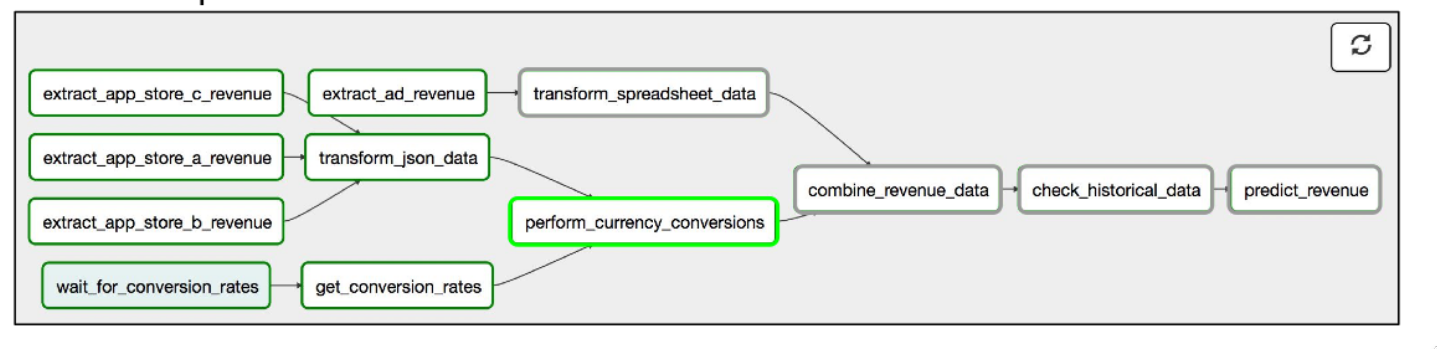
\includegraphics[scale=0.2]{dag_graph_view.png}
  \end{center}
\end{frame}
\begin{frame}[fragile=singleslide]
  \frametitle{Arquitectura}
  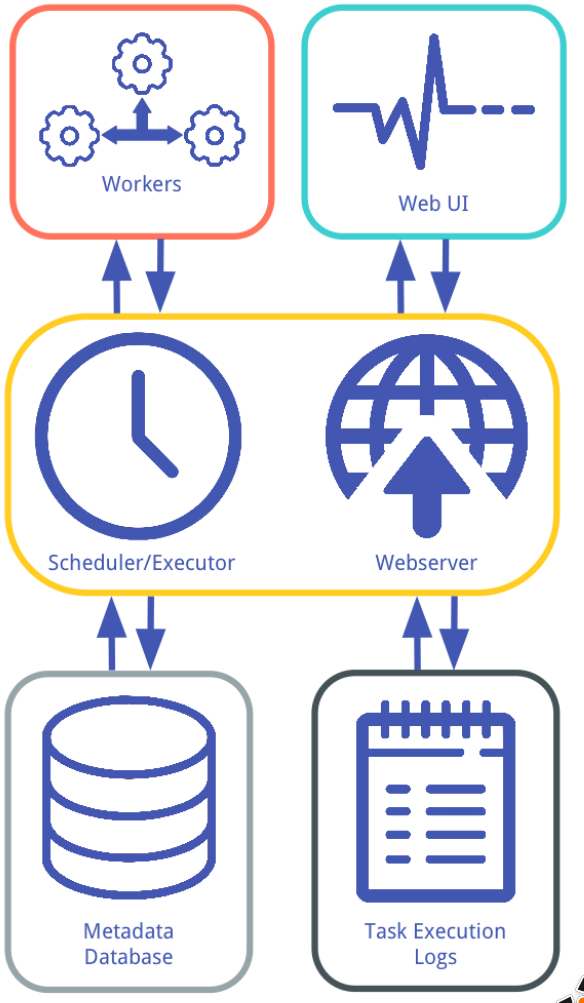
\includegraphics[width=0.22\textwidth]{airflow_architecture.png}%
  \hfill
  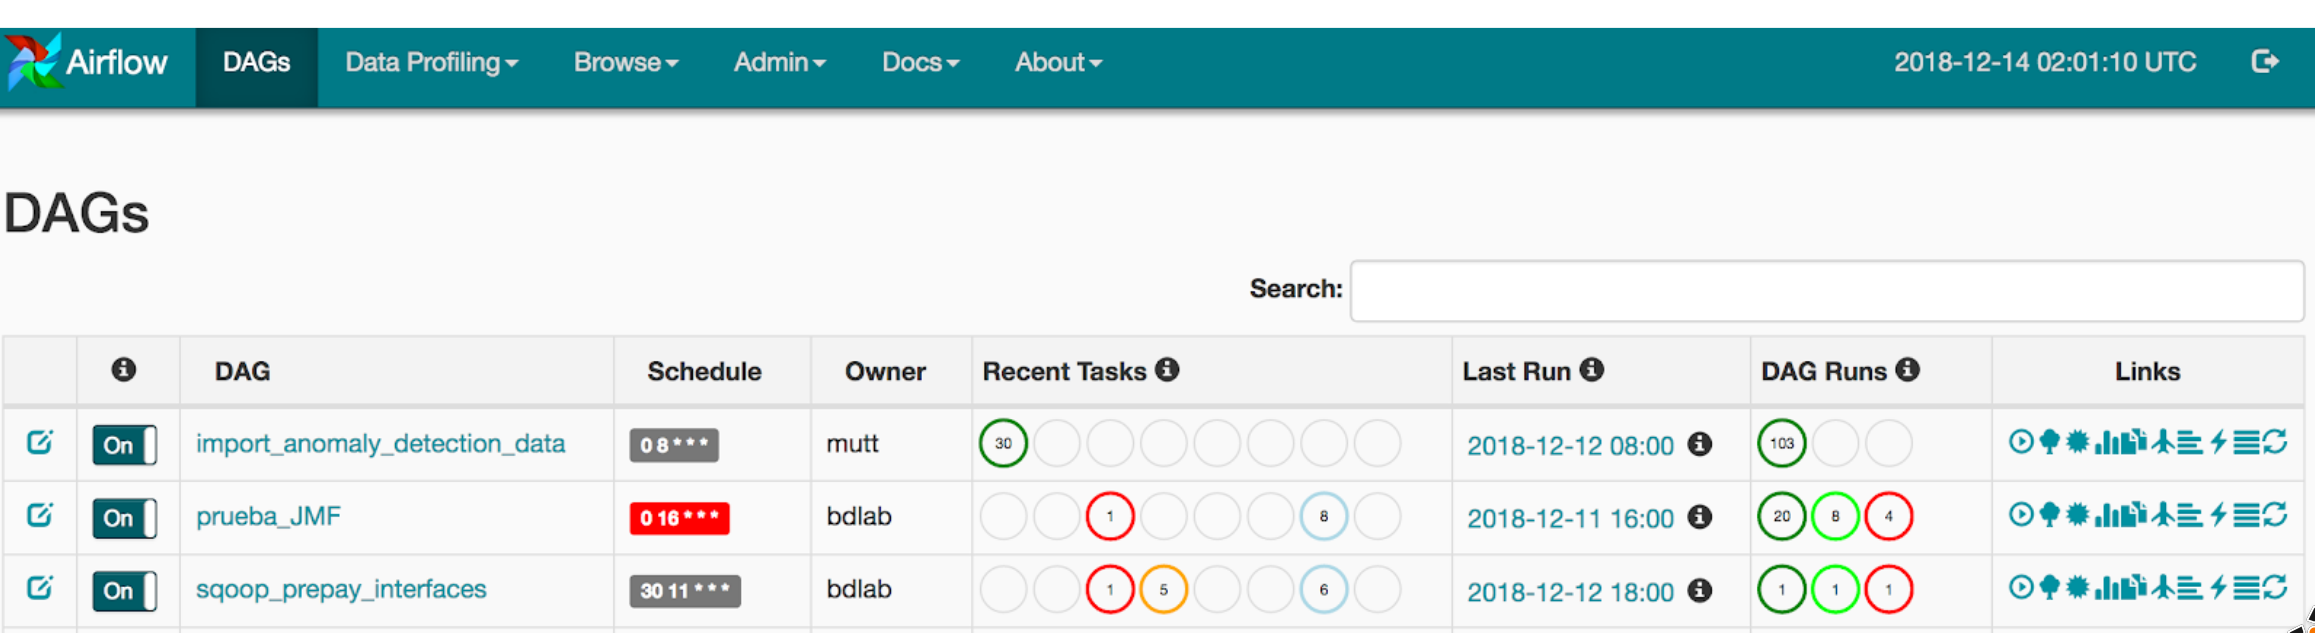
\includegraphics[width=0.75\textwidth]{airflow_ui.png}
  \begin{itemize}
    \item En particular
      \begin{itemize}
        \item Metadata DB: guarda el estado de las tareas y workflows (DAGs)
        \item Scheduler/Executor: scheduler monitorea en forma continua los DAGs y
          inicia las corridas de estos (las tareas son luego ejecutadas por un
          worker determinado por el Executor (cola de mensajes))
        \item Webserver/Logs/UI: El webserver se comunica con la db y
          renderiza el estado de las tareas y logs en la UI.
      \end{itemize}
  \end{itemize}

\end{frame}


\section{DAGs y Ejercicios Guiados}
\label{sec:primeros_dags}


\begin{frame}[fragile=singleslide]
  \frametitle{Digresión: Poetry y Python virtual environments}
  \begin{itemize}
    \item \textit{Poetry} es una herramienta que combina el manejador de
      paquetes \textit{pip} con virtual environments (un directorio con una
      instalacion aislada de Python)
    \begin{itemize}
      \item ¿Cómo lo instalamos?
      \begin{minted}{shell}
      $> python -m pip install --user poetry
      $> which poetry
      /home/pedro/.local/bin/poetry
      \end{minted}
      \begin{itemize}
        \item Si esto devuelve un error agregar \texttt{\$HOME./local} a la
          variable de entorno \texttt{\$PATH}.
      \end{itemize}
      \item ¿Cómo instalamos librerías con poetry?
        \begin{enumerate}
          \item Crear un nuevo directorio airflow-101 y en el correr
          \begin{minted}{shell}
          $> poetry init
          $> poetry add colorful
          \end{minted}
        \item Probemos ahora correr
          \begin{minted}{shell}
          $> python -c "import colorful"
          ModuleNotFoundError: No module named 'colorful'
          $> which python
          /usr/bin/python
          $> poetry run python -c "import colorful"
          \end{minted}
        \item Podemos \textit{spawnear} una nueva shell dentro del venv:
          \begin{minted}{shell}
          $> poetry shell
          (airflow-101) $> which python
          /home/pedro/.cache/pypoetry/virtualenvs/
          \end{minted}
        \end{enumerate}
    \item Notemos además que se creó un archivo \texttt{poetry.lock} que
      especifica los \textit{requerimientos} de librerías para nuestra
        aplicación junto a la versión de Python
    \end{itemize}
  \end{itemize}
\end{frame}
\begin{frame}[fragile=singleslide]
  \frametitle{Instalación local de Apache Airflow}
  \begin{itemize}
    \item Ejecutar los siguientes comandos
      \begin{enumerate}
        \item Instalar apache-airflow
        \begin{minted}{shell}
        $> poetry add apache-airflow
        \end{minted}
        \item Opcional: cambiar el directorio default de configuración de airflow
          (\texttt{~/airflow}) setteando una variable de entorno
          \texttt{AIRFLOW_HOME} en el archivo \texttt{~/airflow-101/.env}:
          \begin{minted}{shell}
          $> echo 'AIRFLOW_HOME="/home/pedro/airflow-cfg"' > .env
          $> cat .env
          AIRFLOW_HOME="/home/pedro/airflow-cfg"
          \end{minted}
          \begin{itemize}
            \item Al correr \texttt{poetry shell} se debe luego
              \textit{sourcear} este archivo con \texttt{source .env}.
          \end{itemize}
        \item Abra una shell de Poetry y corra \texttt{airflow version}, esto
          creara la carpeta con los archivos de configuracion, logs, etc:
          \begin{minted}{shell}
          $> ls ~/airflow-cfg
          $> poetry shell
          (airflow-101) $> source .env && echo $AIRFLOW_HOME
          /home/pedro/airflow-cfg
          (airflow-101) $> airflow version
          (airflow-101) $> ls ~/airflow-cfg
          airflow.cfg airflow.db logs unittests.cfg
          \end{minted}
      \end{enumerate}
  \end{itemize}
\end{frame}
\begin{frame}[fragile=singleslide]
  \frametitle{Instalación local de Apache Airflow II}
  \begin{itemize}
    \item Continuar ejecutando los siguientes comandos
    \begin{enumerate}
      \setcounter{enumi}{3}
      \item Cree
        nuevo directorio \texttt{dags} (aquí guardaremos el archivo
        \texttt{titanic_dag.py} definido en el siguiente slide) y cambie el directorio de dags
        (\texttt{dags_folder}) en
        \texttt{~/airflow-cfg/airflow.cfg} para que apunte a este nuevo
        directorio:
      \begin{minted}{shell}
      $> mkdir dags && cd dags
      ...
      $> head ~/airflow-cfg/airflow.cfg | grep dags_folder
      dags_folder = /home/pedro/airflow-101/dags
      \end{minted}
    \item Corra dentro de la shell de Poetry \texttt{airflow initdb} y luego \texttt{airflow list_dags}
      para listar los dags.
    \item Corra \texttt{airflow webserver -p 9594} y abra \texttt{localhost:9594} en
      el browser
    \item Inspeccione los dags: para correrlos debe activarlos y luego
      prender el scheduler con \texttt{airflow scheduler}
    \end{enumerate}
  \end{itemize}
  \begin{center}
    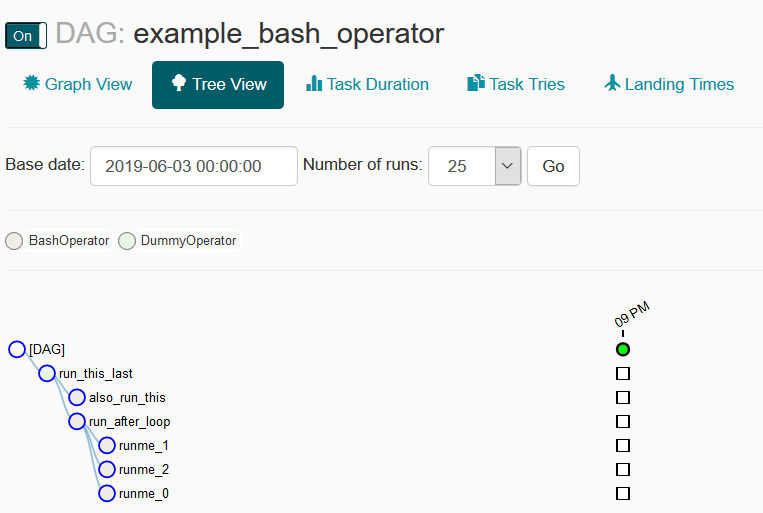
\includegraphics[scale=0.2]{example_bash_operator.png}
  \end{center}
\end{frame}
\begin{frame}[fragile=singleslide]
  \frametitle{Nuestro primer dag: Bash, Dummy y Python Operators}
  \begin{minted}{python}
from datetime import datetime
from pathlib import Path
from airflow.models import DAG
from airflow.operators.bash_operator import BashOperator
from airflow.operators.dummy_operator import DummyOperator
from airflow.operators.python_operator import PythonOperator

STORE_DIR = Path(__file__).resolve().parent / 'tmp-files' / 'random-num'
Path.mkdir(STORE_DIR, exist_ok=True, parents=True)
bash_cmd = f"echo $(( ( RANDOM % 10 )  + 1 )) > {str(STORE_DIR / 'random_number.txt')}"

def _read_number_and_square(store_dir):
    fn = str(store_dir / 'random_number.txt')
    with open(fn, 'r') as f:
        n = f.readline()
    return int(n) ** 2

default_args = {'owner': 'pedro', 'retries': 0, 'start_date': datetime(2020, 4, 10)}
with DAG(
    'random_number', default_args=default_args, schedule_interval='0 4 * * *'
) as dag:
    dummy_start_task = DummyOperator(task_id=f'dummy_start')
    generate_random_number = BashOperator(
        task_id='generate_random_number', bash_command=bash_cmd)
    read_num_and_square = PythonOperator(
        task_id='read_number_and_square_it',
        python_callable=_read_number_and_square,
        op_args=[STORE_DIR])
    dummy_start_task >> generate_random_number >> read_num_and_square
  \end{minted}

\end{frame}
\begin{frame}[fragile=singleslide]
  \frametitle{Exercise 1: Extending random number dag}
  \begin{enumerate}
    \item Using the random_number_dag.py file do the following steps in order
      to build the workflow seen in the figure
    \begin{enumerate}
      \item Add logging messages that signal a) which file is going to be read and b) what number was read from the file.
      \item The filename is currently hardcoded as random_number.txt, change it
        to reflect the execution date i.e files should now be named something
        like 20200413.txt. \textit{Hint}: you need to capture the execution date by
        adding a **context arg in the Python callable.
      \item Hard: convert the PythonOperator into a BranchPythonOperator that will be followed by another PythonOperator (BashOperator) task that prints HIGH (LOW) if the resulting squared numbered is greater (smaller) than 30.
      \item Extra (take-home): Add logic to erase the created temporary files.
    \end{enumerate}
  \end{enumerate}
  \begin{center}
    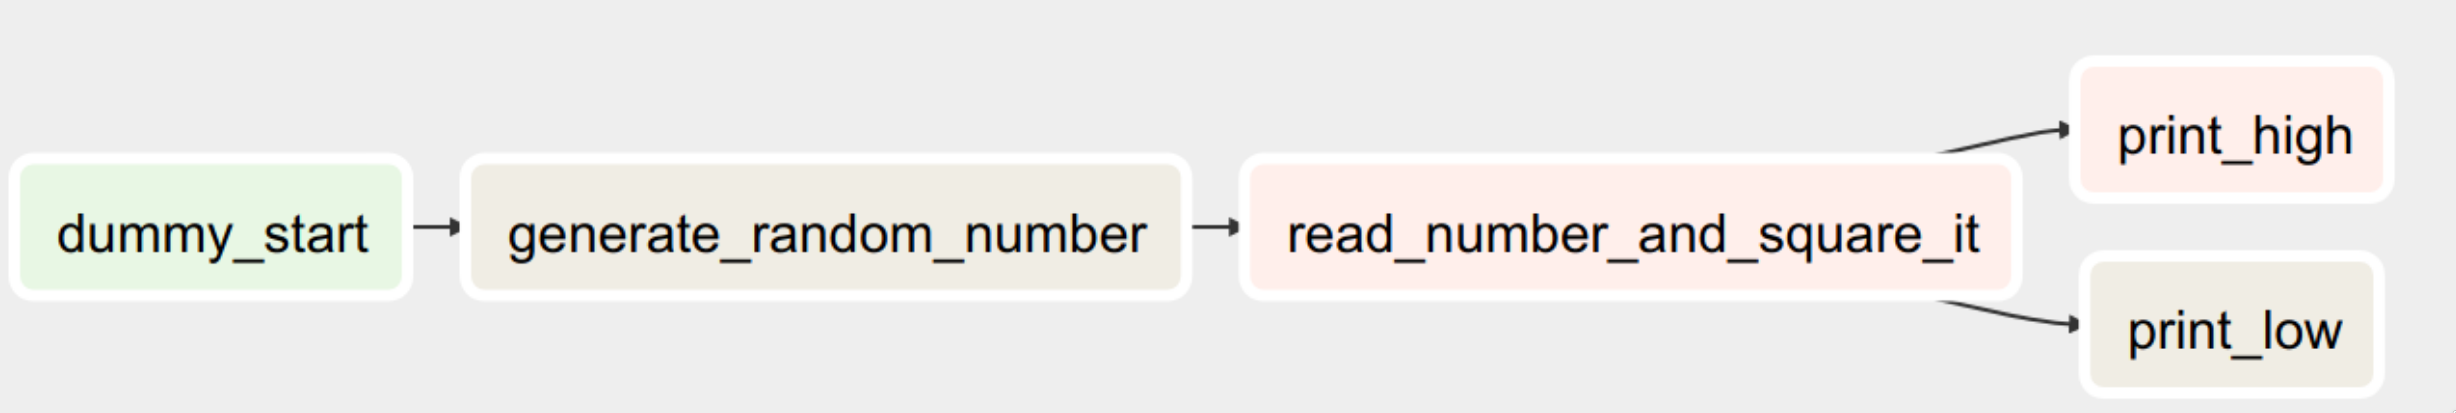
\includegraphics[scale=0.1]{exercise_1.png}
  \end{center}
\end{frame}
\begin{frame}[fragile=singleslide]
  \frametitle{Segundo dag: insertando a db con xcoms}
  \begin{itemize}
    \item Opcional: Realicemos los siguientes pasos antes de correr el dag
      \texttt{stocks_dag.py}:
      \begin{enumerate}
        \item Instalemos una cli de sqlite llamada \texttt{litecli} con \texttt{pip}:
        \begin{minted}{shell}
        $> pip install litecli
        $> ~/.local/bin/litecli /tmp/sqlite_default.db
        \end{minted}
      \item Chequeamos que \texttt{stocks_dag} aparece listado por
        \texttt{airflow list_dags}
        \begin{itemize}
          \item Si ello no sucede podemos resettear la db con \texttt{airflow
            resetdb} (cuidado con este comando!)
        \end{itemize}
      \item Activar el dag y dejarlo correr por el scheduler
      \item Completadas las tareas chequear que los datos se insertaron desde
        la cli de sqlite o a través del objeto \texttt{SqLiteClient} de Python.
        \begin{minted}{shell}
        $> ~/.local/litecli /tmp/sqlite_default.db
        /tmp/sqlite_default.db> select * from stocks_daily;
        +------------+--------+--------------------+-----------+
        | date       | symbol | avg_num_trades     | avg_price |
        +------------+--------+--------------------+-----------+
        | 2020-04-08 | aapl   | 29322.097916666666 | 264.3     |
        | 2020-04-09 | aapl   | 28145.224305555555 | 267.385   |
        | 2020-04-10 | aapl   | <null>             | <null>    |
        \end{minted}
      \end{enumerate}
    \item Notar algunos elementos importantes del dag
      \begin{itemize}
        \item El \textit{execution_date} es el período de tiempo en el cual
          vamos a procesar la data (distinto del período/momento de la corrida)
        \item Si volvemos a correr uno de los tasks de inserción el dag
          rompe...
      \end{itemize}
  \end{itemize}
\end{frame}
\begin{frame}[fragile=singleslide]
  \frametitle{Exercise 2: Small Stocks report}
  \begin{enumerate}
    \item Using the stock_dag.py file do the following steps in order to build the
workflow seen in the figure
    \begin{enumerate}
      \item Modify the workflow to also get (and insert) data from Tesla (tsla)
        and Facebook (fb) stocks. Note: the easy way to do this is to add a
        loop inside the method that performs the request. The harder one (
        seen in the figure) is to have one branch
        per company spawning from the initial task which then reunite in the
        insert task.
      \item Note that if you clear an insert task and re-run it you'll get an
        error (due to the unique constraint). Add some try/catch logic to
        gracefully avoid this error in the insert callback function.
        \begin{enumerate}
          \item You can alternatively let the task fail and add trigger_rule='all_done' to the
        successive task in order to trigger it regardless of the failure of the previous task.
        \end{enumerate}
      \item Add a new task that reads (i.e queries) all records inserted in the present run and returns a string stating which was the company with the highest average trades per minute in that date.

      \item Bonus: Create a final task that sends an email, using EmailOperator, of the
report/insight obtained in 3.  Note: for this exercise you will need to modify the
smpt entry in the airflow.cfg file
        \end{enumerate}
        \end{enumerate}
    \begin{center}
       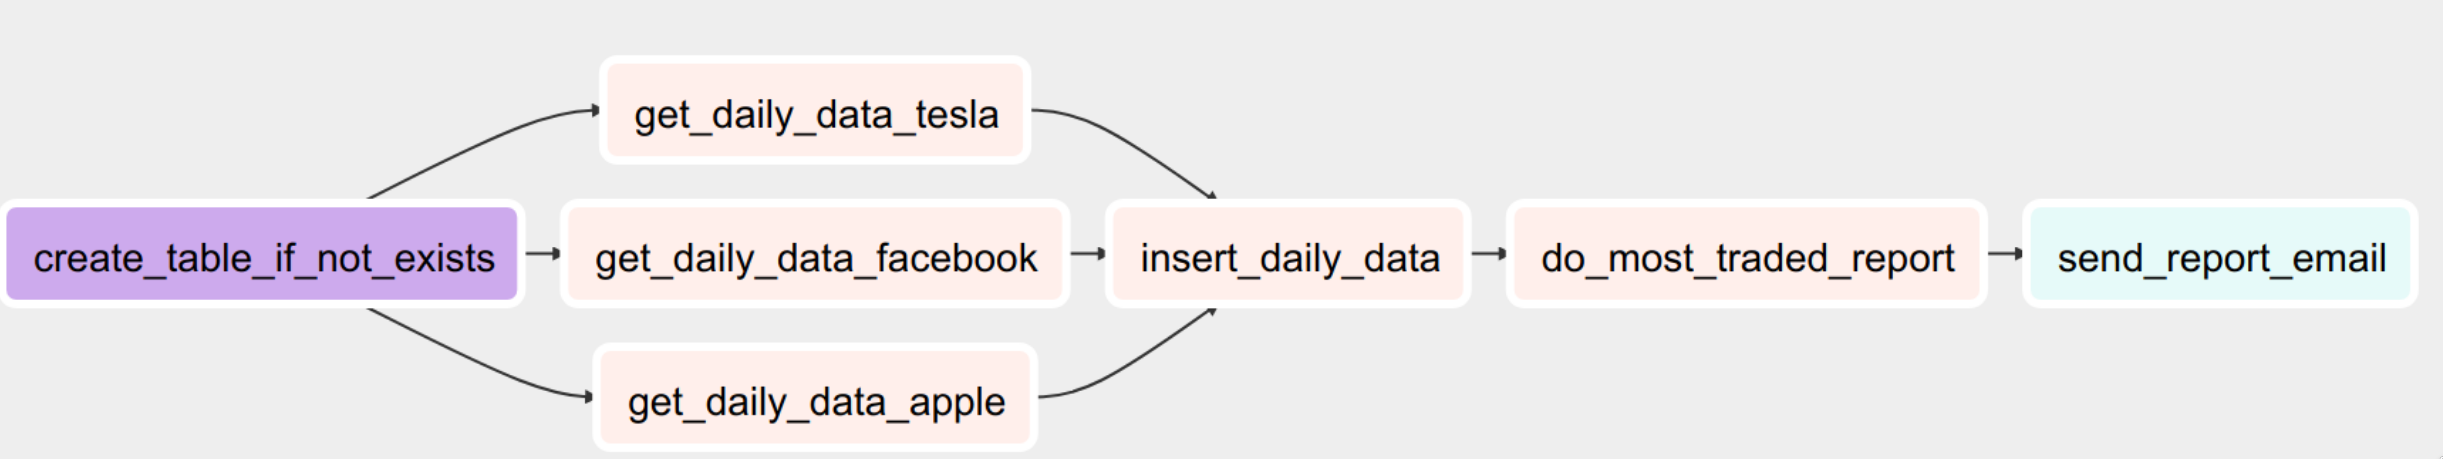
\includegraphics[scale=0.1]{exercise_2.png}
    \end{center}
\end{frame}

\section{Ejercicios Adicionales}
\label{sec:ejercicios_adicionales}

\begin{frame}[fragile=singleslide]
  \frametitle{Exercise 3 (MEDIUM): Scheduling Titanic Prediction}
  \begin{enumerate}
    \item (Optional) Install a local version of Airflow following the previous
      slides.
    \item The previous class we solved Kaggle's Titanic Disaster Prediction
      Challenge using an \enquote{ETFL} pipeline. In this exercise you are
      requested to schedule such pipeline with Airflow using what you've learnt
      in the past two exercises. The objective is to create a DAG from scratch
      that defines a workflow like the one shown in the image.
    \begin{enumerate}
      \item Create PythonOperators that perform the following sequential task
        \begin{itemize}
          \item Extraction of Titanic data.
          \item Trasnformation of such data.
          \item Fit a Random Forest to the transformed data.
          \item Load results into a csv file.
        \end{itemize}
    \begin{enumerate}
          \item Bonus: In order to have some variability in runs between different
            dates hash the execution date as use that as the random number
            generator seed.
          \item Bonus: Load predictions into a DB of your choice.
        \end{enumerate}
      \end{enumerate}
      \end{enumerate}
  \begin{center}
    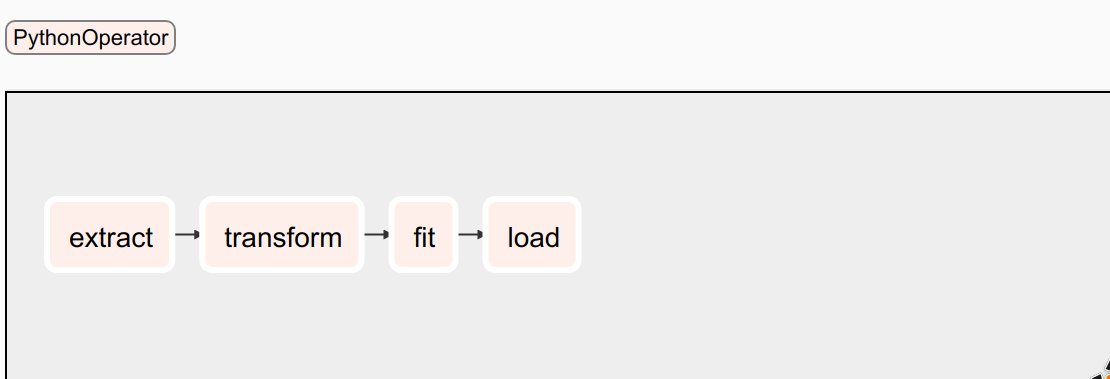
\includegraphics[scale=0.2]{exercise_3.png}
  \end{center}
\end{frame}
\begin{frame}[fragile=singleslide]
  \frametitle{Exercise 4 (HARD): DockerOperator and SQLSensor}
  \begin{enumerate}
    \item Uncomment the commented code in \texttt{word\_count_dag.py} and try to
      fix the resulting error when loading the dag. \texttt{Hint}: you need to
      install the Python \texttt{docker} library.
    \item The \texttt{word\_count_dag.py} DAG launches a Spark job via
      \texttt{DockerOperator} to find out which is the most recurring word in a
      text file. This is then inserted in a SQL table. You can check out the
      Spark file at \texttt{spark_job.py}.  Follow the next steps to build the
      workflow seen in the figure.
    \begin{enumerate}
      \item Create a connection to a valid Postgres database. You can do this
        through the Airflow UI via Admin -> Connections. Remember to properly
        set your connection ID in your operators.
      \item The Spark job can read the environment variables
        \texttt{INPUT\_FILE} and \texttt{OUTPUT\_FILE} to know which file to
        count words from and which to store its result respectively. Use
        DockerOperator's environment variables to set these variables to an
        input file of your liking and an output file with a dynamic filename
        like: \texttt{<EXECUTION\_DATE>.csv}. Also try to keep the working
        environment clean of files!
      \item Create a PythonOperator to get a text file of your liking to use as
        \texttt{INPUT\_FILE}. For example, checkout
        \href{https://wikipedia.readthedocs.io/en/latest/code.html}{wikipedia's
        API}.
      \item Create a SqlSensor which pokes the database and checks if a certain
        keyword was the most used word. If it was, launch a new task.
    \end{enumerate}
  \end{enumerate}
  \begin{center}
    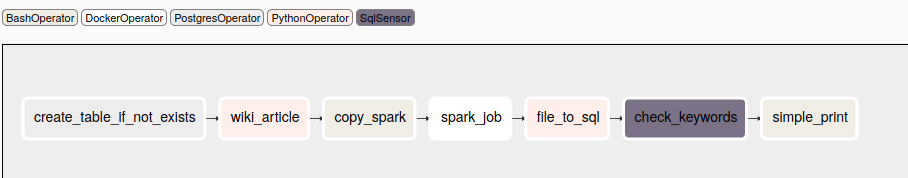
\includegraphics[scale=0.2]{exercise_4.png}
  \end{center}
\end{frame}

\begin{frame}[fragile=singleslide]
  \frametitle{Referencias}
  \begin{itemize}
    \item Maxime Beauchemin (creador de Airflow)
      \begin{itemize}
        \item \href{https://www.freecodecamp.org/news/the-rise-of-the-data-engineer-91be18f1e603/}{The Rise of the Data Engineer}
        \item \href{https://medium.com/@maximebeauchemin/the-downfall-of-the-data-engineer-5bfb701e5d6b}{The Downfall of the Data Engineer}
        \item \href{https://medium.com/@maximebeauchemin/functional-data-engineering-a-modern-paradigm-for-batch-data-processing-2327ec32c42a}{Functional Data Engineering}
      \end{itemize}
    \item \href{https://medium.com/@dustinstansbury/beyond-cron-an-introduction-to-workflow-management-systems-19987afcdb5e}{Quizlet Beyond Cron Series}
    \item \href{https://www.astronomer.io/guides/}{Astronomer Apache Airflow Guides}
  \end{itemize}
\end{frame}
\end{document}
